\documentclass[11pt]{article}
\usepackage{amsmath}
\usepackage{amsthm}
\usepackage{amsfonts}
\usepackage[margin=1in]{geometry}
\usepackage{amssymb}
\usepackage{graphicx}

\newcommand{\xx}{\vec{x}}
\newcommand{\cc}{\vec{c}}
\newcommand{\bb}{\vec{b}}
\newcommand{\uu}{\vec{u}}
\newcommand{\vv}{\vec{v}}
\newcommand{\vgg}{\vec{g}}
\newcommand{\rr}{\vec{r}}

\newcommand{\matlab}{\textsc{Matlab\ }}    
\newcommand{\matlabns}{\textsc{Matlab}}  

\title{CPSC 302, Fall 2022, Assignment 5}
\author{Released Thursday, November 24, 2022 \\
Due Monday, December 5, 2022, 11:59pm}
\date{}
\begin{document}
\maketitle 

%%% Question 1
\begin{enumerate}
\item Consider the $2 \times 2$ matrix
$$
A=\left( \begin{array}{cc}
2 & -1   \\
-1 & 2  \\
\end{array} \right)
\ ,
$$
and suppose we are required to solve $A \xx=\bb$, where $\bb$ is an arbitrary right-hand side vector. Clearly, solving a $2
\times 2$ linear system using a stationary scheme is an utterly ridiculous idea,
but the following is helpful in understanding
 more about convergence  of stationary methods.
\begin {enumerate}
\item Find the spectral radius of the Jacobi and
Gauss-Seidel iteration matrices and the asymptotic rate of
convergence for these two schemes, namely $-\log_{10} \rho(T)$, where $\rho(T)$ denotes the spectral radius of the corresponding iteration matrix, $T$. 
\item How much faster does Gauss-Seidel converge compared to Jacobi for a fixed reduction in the relative residual norm, $\frac{\| \rr_k \|_2}{\| \bb \|_2}$, in terms of iteration counts?
\item Write down the SOR iteration matrix as a function of the relaxation parameter, $\omega$.  
\item Find the optimal SOR parameter, $\omega_{\rm opt}$,
and the spectral radius of the corresponding iteration matrix.
\item Approximately how much faster does SOR with $\omega_{\rm opt}$ converge
compared to Jacobi?
\end{enumerate}

%%% Question 2
\item 
\begin{enumerate}
\item Download from the assignment webpage the file {\tt J\_GS.m}. In your {\sc Matlab} command line, run the command: {\tt J\_GS(100);} \\
%\begin{verbatim}
%J_GS(100); 
%\end{verbatim}
Include in your assignment solution the convergence graph that you are seeing. This is a linear system with the two-dimensional Laplacian of size $10,000 \times 10,000$ (we have $n=100, n^2=10,000$), and we are plotting the norm of the relative residual after 10,000 iterations for Jacobi and Gauss-Seidel. There is no reason to be impressed with this graph; convergence here is slow. But we are going to see  the effect of using SOR.
\item Given the eigenvalues of the Laplacian in the slides, show that the optimal SOR parameter can be expressed as
$$ \omega_{\rm opt} = \frac{2}{1+\sin \left( \frac{\pi}{n+1} \right)}.$$
\item
Modify the  {\sc Matlab} function so that in addition to the Jacobi and Gauss-Seidel graphs (for the same matrix) a convergence plot for the SOR method is included as well. Use the same initial guess (the zero vector) and the same stopping criterion: $\frac{\| \rr_k \|_2}{\| \bb \|_2} < 10^{-6}$. 

{\underline {Tip}:} You should be seeing an {\em extremely dramatic} improvement in convergence. If you are not seeing such an improvement, then you must have done something wrong.
\item Explain your results. 
\end{enumerate}

%%% Question 3
\item \begin{enumerate}
\item Suppose $A$ is an $n$-by-$n$ orthogonal matrix.
Show that all its singular values are equal to 1.
\item Recall that an orthogonal projector is a symmetric matrix $P$
for which $P^2=P$.
What are the eigenvalues of an orthogonal projector?
\end{enumerate}

%%% Question 4
\item Load the following .mat matrix that appears on the assignment page:
\begin{verbatim}
load powerMatrix;
\end{verbatim}
If you hit {\tt whos} you should be seeing a matrix called $A$, of size $100 \times 100$. To validate any of your results below, you may run the {\sc {Matlab}} command {\tt eig}, as long as you understand that in typical eigenvalue computations (in a potentially more challenging computational environment) we generally do not have the luxury of running  {\tt eig} to check ourselves. 
\begin{enumerate}
\item Apply the power method. Terminate the iteration once the iterates satisfy
$$|\lambda_1^{(k)}-\lambda_1^{(k-1)}| < 10^{-4}.$$ Your program should
print out the value of the final iterate and a graph of the absolute errors:
$| \lambda_1^{(k)}-\lambda_{\max}|$. For better visualization, use {\tt semilogy}  for your graphs
when necessary. As an
initial guess for the eigenvector use a vector produced by the
\textsc{Matlab} command {\tt randn}. (When you repeat your experiments, the number of iterations may slightly vary due to the random initial guess.)
\item Repeat your computations with the {\em inverse} power
iteration, with a shift $\alpha=4$, and produce the same graph as
you did for the power method.
\item Discuss the differences between the performance of
the power and the inverse power methods in terms of the cost of single iterations and the overall 
computational cost.
\item Suppose now that we know that $A$ has an eigenvalue close to 3 and we are interested to compute it to six correct decimal digits. Suggest an efficient procedure for doing so. Implement your suggested algorithm and compute the eigenvalue.
\end{enumerate}

%%% Question 5
\item The following picture appears in \textsc{Matlab's}
repository of images, and can be retrieved by entering 
\begin{verbatim}
load mandrill;
colormpap(`gray');
image(X);
\end{verbatim}

\begin{center}
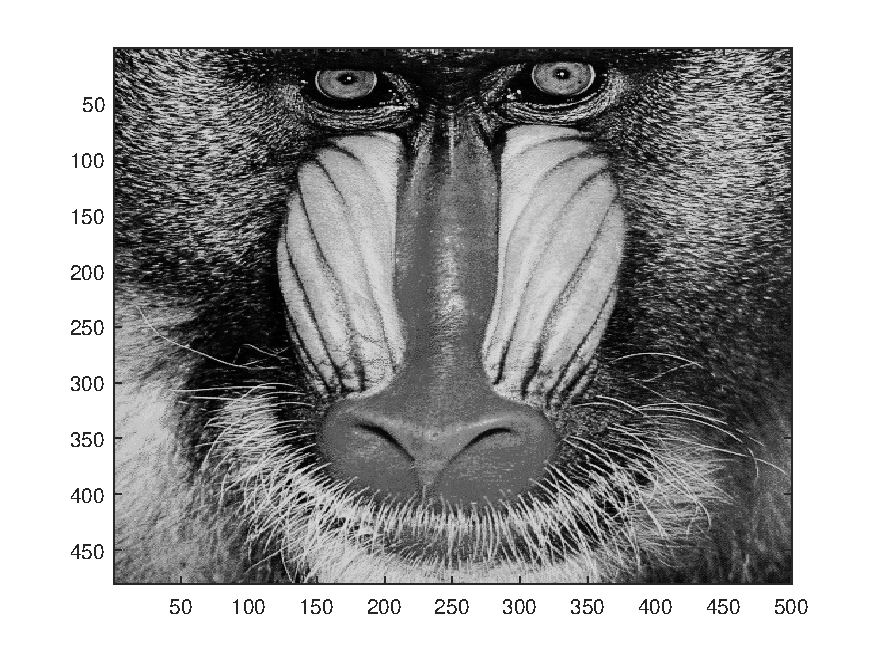
\includegraphics{mandrill2.pdf}
\end{center}

\begin{enumerate}
\item
Print out
the images generated by the truncated SVD. Start
with $r=2$ and go up by powers of $2$, to $r=2^6=64$ (six plots in total). For a compact
presentation of your figures, you may use the command
{\tt subplot(3,2)}. (Check out {\tt help subplot}.)

\item Comment briefly on the quality of the images as a function of $r$. For what value of $r$ would you say that the quality of the image is acceptable, in that we can be rather confident of what we are seeing? (We are not looking for a specific ``correct answer'' here - just make your subjective observation.)
\item For the value of $r$ you stated in part (b), how much storage is required? Compare it to the storage required for the original image.
\end{enumerate}


\end{enumerate}
\end{document}
​